\documentclass{article}
\usepackage{amsmath}
\usepackage{listings}
\usepackage{moreverb}
\usepackage[margin=1in]{geometry}
\usepackage{graphicx}
\usepackage{dsfont}
\title{STA 360: Assignment 3}
\author{Michael Lin}

\begin{document}
\maketitle

\begin{enumerate}
\setcounter{enumi}{1}

\item Since $Z$ has distribution Binomial$(n,\theta)$, the p.d.f. of $z$ is:
\begin{align*}
p(z|\theta) &= {n \choose z} \theta^z(1-\theta)^{n-z} \mathds{1}(z\in S)\\
&={n \choose z} \exp \{ \log[\theta^z(1-\theta)^{n-z}] \} \mathds{1}(z\in S)\\ 
&={n \choose z} \exp \{\log\theta^z+\log(1-\theta)^{n-z} \} \mathds{1}(z\in S)\\
&={n \choose z} \exp \{z\log\theta+(n-z)\log(1-\theta) \} \mathds{1}(z\in S)\\
&={n \choose z} \exp \{z\log\theta+n\log(1-\theta)-z\log(1-\theta) \} \mathds{1}(z\in S)\\
&={n \choose z} \exp \{z\log\frac{\theta}{1-\theta}+n\log(1-\theta) \} \mathds{1}(z\in S)\\
&={n \choose z} \exp \{z\log\frac{\theta}{1-\theta}-n\log\frac{1}{1-\theta} \}\mathds{1}(z\in S)
\end{align*}
where $S = \{0,1,2,...,n\}$. From here, we see that:
\begin{align*}
t(z)&=z \\
\phi(\theta)&=\log\frac{\theta}{1-\theta} \\
\kappa(\theta) &= n\log\frac{1}{1-\theta} \\
h(z)&={n \choose z} \mathds{1}(z\in S)
\end{align*}
Thus, for a fixed $n$ and given parameter $\theta$, Binomial$(n,\theta)$ distributions form a one-parameter exponential family.

\item Given that the generating distribution is $p(x|a,b)=\text{Gamma}(x|a,b)$ where $a$ is fixed, the form of this distribution is:
\begin{align*}
p(x_{1:n}|b) &= \prod\limits_{i=1}^{n} \frac{b^a}{\Gamma(a)} x_i^{a-1}e^{-bx_i} \\
&\propto b^{an}e^{-b\sum x_i} \\
\end{align*}
We will show that a conjugate prior for $b$ is $p(b) = \text{Gamma}(b|\alpha,\beta)$ by considering the corresponding posterior distribution.
\begin{align*}
p(b|x_{1:n})&=p(b)p(x_{1:n}|b) \\
&\propto \frac{\beta^\alpha}{\Gamma(\alpha)}b^{\alpha-1}e^{-\beta b}b^{an}e^{-b\sum x_i} \\
&\propto b^{(\alpha+an)-1}e^{-b(\beta+\sum x_i)} \\
&\propto \text{Gamma}(b|\alpha+an,\beta+\sum x_i)
\end{align*}
Since the posterior, like the prior, is also a Gamma distribution, thus $p(b) = \text{Gamma}(b|\alpha,\beta)$ is a conjugate prior for $b$.

\setcounter{enumi}{4}
\item Given conjugate prior $p_{n_0,t_0}(\theta)$ and i.i.d. probability distributions $p(x|\theta)$, the posterior distribution $p(\theta|x_{1:n})$ is the following:
\begin{align*}
p(\theta|x_{1:n}) &= p_{n_0,t_0}(\theta) \prod\limits_{i=1}^{n} p(x_i|\theta) \\
&\propto \exp\{n_0t_0\phi(\theta)-n_0\kappa(\theta)\} \prod\limits_{i=1}^{n} \{\exp(\phi(\theta)t(x_i) - \kappa(\theta))h(x_i) \}\\
&=\exp\{n_0t_0\phi(\theta)-n_0\kappa(\theta)\} [\prod\limits_{i=1}^{n}h(x_i)]\exp\{\sum\limits_{i=1}^{n}(\phi(\theta)t(x_i) - \kappa(\theta)) \} \\
&\propto \exp\{n_0t_0\phi(\theta)-n_0\kappa(\theta)\} \exp\{\sum\limits_{i=1}^{n}(\phi(\theta)t(x_i) - \kappa(\theta)) \} \\
&=\exp\{n_0t_0\phi(\theta)-n_0\kappa(\theta) + \phi(\theta)\sum\limits_{i=1}^{n} t(x_i) - n\kappa(\theta) \} \\
&=\exp\{ (n_0t_0+\sum\limits_{i=1}^{n}t(x_i))\phi(\theta)-(n_0+n)\kappa(\theta)\}\\
&=\exp\{(n_0+0)\frac{n_0t_0+\sum\limits_{i=1}^{n}t(x_i)}{n_0+n} \phi(\theta) - (n_0+n)\kappa(\theta) \} \\
&=\exp\{n't'\phi(\theta)-n'\kappa(\theta)\} \\
&\propto p_{n',t'}(\theta)
\end{align*}
where $n'=n_0+n$ and
$$ t'=\frac{n_0t_0+\sum\limits_{i=1}^{n}t(x_i)}{n_0+n}$$

\setcounter{enumi}{6}
\pagebreak
\item See image below: \\
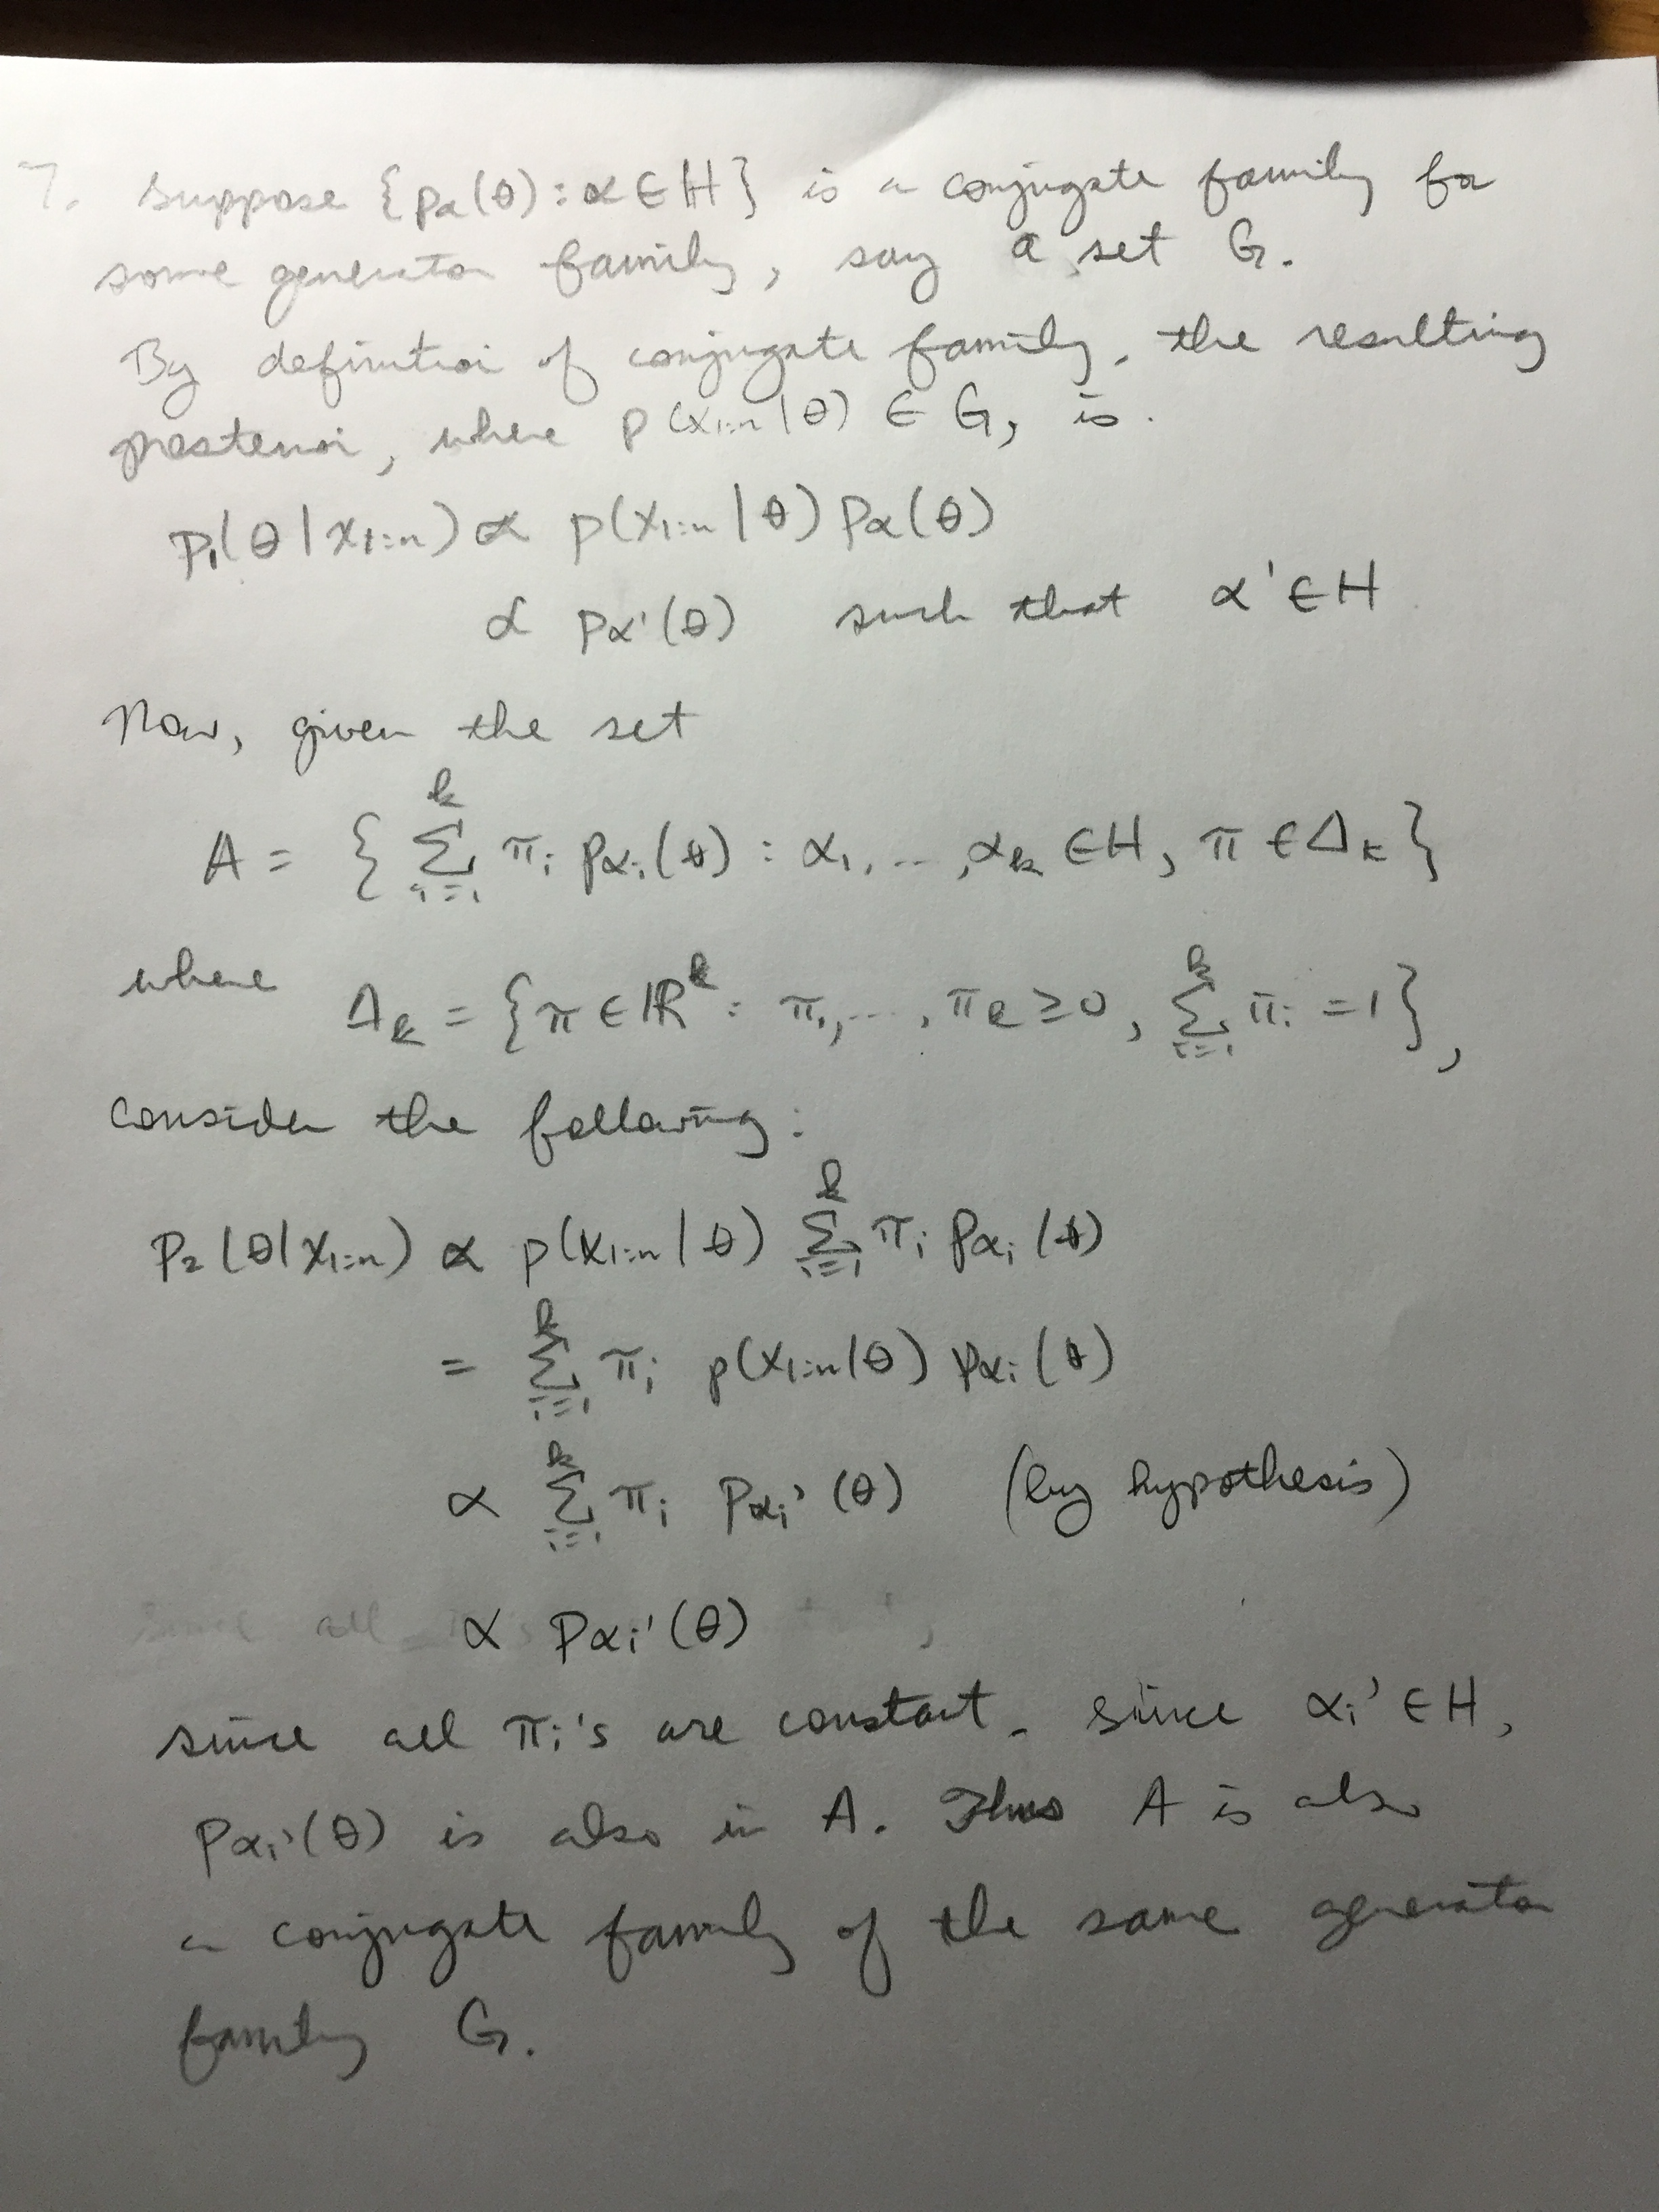
\includegraphics[scale=0.18]{pic.jpg}

\end{enumerate}

\pagebreak
Additional exercise: Given prior distribution $p(\theta)$ and generated distribution $p(x|\theta)$, the posterior distribution is as follows:

\begin{align*}
p(\theta|x_{1:n})&=p(x_{1:n}|\theta)p(\theta) \\
&=\Big\{\prod\limits_{i=1}^{n}\sqrt{\frac{\lambda}{2\pi}}\exp(-\frac{\lambda}{2}(x_i-\theta)^2)\Big\} \sqrt{\frac{\lambda_0}{2\pi}} \exp(-\frac{\lambda_0}{2}(\theta-\mu_0)^2) \\
&\propto \exp(-\frac{\lambda}{2}\sum\limits_{i=1}^{n}(x_i-\theta)^2)\exp(\frac{\lambda_0}{2}(\theta-\mu_0)^2) \\
&=\exp(-\frac{1}{2}[\lambda\sum\limits_{i=1}^{n}(x_i-\theta)^2+\lambda_0(\theta-\mu_0)^2])\\
&=\exp(-\frac{1}{2}[\lambda\sum\limits_{i=1}^{n}(x_i^2-2x_i\theta+\theta^2)+\lambda_0(\theta^2-2\theta\mu_0+\mu_0^2)])\\
&=\exp(-\frac{1}{2}[\lambda\sum\limits_{i=1}^{n}x_i^2-2\lambda\theta\sum\limits_{i=1}^{n}x_i+n\lambda\theta^2+\lambda_0\theta^2-2\lambda_0\theta\mu_0+\lambda_0\mu_0^2]) \\
&\propto \exp(-\frac{1}{2}[(n\lambda+\lambda_0)\theta^2-2(\lambda\sum\limits_{i=1}^{n}x_i+2\lambda_0\mu_0)\theta])\\
&=\exp(-\frac{n\lambda+\lambda_0}{2}[\theta^2-2(\frac{\lambda\sum\limits_{i=1}^{n}x_i+2\lambda_0\mu_0}{n\lambda+\lambda_0})\theta]) \\
& \propto \exp(-\frac{n\lambda+\lambda_0}{2}(\theta-\frac{\lambda\sum\limits_{i=1}^{n}x_i+2\lambda_0\mu_0}{n\lambda+\lambda_0})^2) \\
&=\exp(-\frac{L}{2}(\theta-M)^2) \\
&\propto \text{Normal}(\theta|M,L^{-1})
\end{align*}
where $L=n\lambda+\lambda_0$ and
$$M=\frac{\lambda\sum\limits_{i=1}^{n}x_i+2\lambda_0\mu_0}{n\lambda+\lambda_0}$$
\end{document}